\documentclass[a4paper,12pt,titlepage]{article}
\usepackage{graphicx}



\DeclareGraphicsExtensions{.jpg}
\graphicspath{{./Images/}}

\begin{document}
	\newcommand{\HRule}{\rule{\linewidth}{0.5mm}}
\begin{titlepage}
\begin{center}

\includegraphics[width = 0.3\textwidth]{US_logo.png}~\\[1cm]
\textsc{\LARGE Unsolvable Solutions}\\
Client: Francois Mouton at the CSIR DSSR\\[1.5cm]
\textsc{\Large  Functional Requirements}\\[0.5cm]

 \HRule\\[0.4cm]
{ \huge \bfseries  Eavesdropping Protection in Conclave \\[0.4cm] }

 \HRule\\ 



Github link:  \url{https://github.com/Unsolvable-Solutions/Project-EPIC} \\[1.2cm]

\noindent
\begin{minipage}[t]{0.4\textwidth}

	\begin{flushleft} \large
	\emph{Members:}\\
		Edwin Fullard  \\
		Jaco Bezuidenhoudt \\
		Jandre Coetzee\\
		Maret Stoffberg\\
		Ryno Pierce\\
	\end{flushleft}
\end{minipage}%
\begin{minipage}[t]{0.4\textwidth}
\begin{flushright} \large
	\emph{Student Number:} \\
		12048675 \\
		11013878 \\
		 10693077 \\
		 11071762 \\
		 12003922\\
	\end{flushright}
\end{minipage}

\vfill


% Bottom of the page




\end{center}
\end{titlepage}




	
	% Table of content
	\newpage
	\tableofcontents
	\newpage
	\section{Introduction}
		\subsection{Project Background}

The Android Operating System officially took over the smartphone market in 2010 and it is suspected that about 700 000 Android devices are used in South Africa. It is mostly the corporate or more upper class communities that have access to these smartphone devices. It is also these individuals who sit in the big corporate meetings where extremely sensitive data can be discussed. For this reason, if these individuals should have eavesdropping malware on their smartphone, it could cause sensitive data to be easily leaked out.


		\subsection{Project Vision}
This project consist of two unique parts: the eavesdropping malware and the protection against it.
		\subsection{Project Scope}
This EPIC (Eavesdropping Protection in Conclave) project consist of a server, an Android application and a gateway device. The android device is held over the gateway node and, using NFC, a request to enter the meeting is send to the server via the gateway device. The server then respond with permission or denial. If permission is granted, the android device will proceed into protection mode and the meeting log is updated. After the meeting has been held, the device will then be held over the gateway node again to deactivate the protection mode. A user may query the log of a meeting.
\newline
The eavesdropping malware use a server and an application on the android device. Ideally the application will be hidden behind another application, but for the sake of this project it will be a visible application. A user will send an eavesdropping request from the server to a specified android device. If this device have the malware installed, it will start streaming the recording to the user. The user may then send a request to stop the recording and store the recording.

	%  The functional requirements
\newpage
	\section{Functional Requirements}
	
		\subsection{Server}
		\textbf{Scope: } 	The server is used with the gateway, it sends and receives data to and from the gateway. On the server an administrative user must also be able to add, remove, edit and view the users, administrative users included. Any user must be able to log in and log out of the system on the server. When logged in the user may create, update, delete and request summary from a meeting. The user may also view and edit his own profile.
		\begin{figure}[h!]
 			 \centering
			  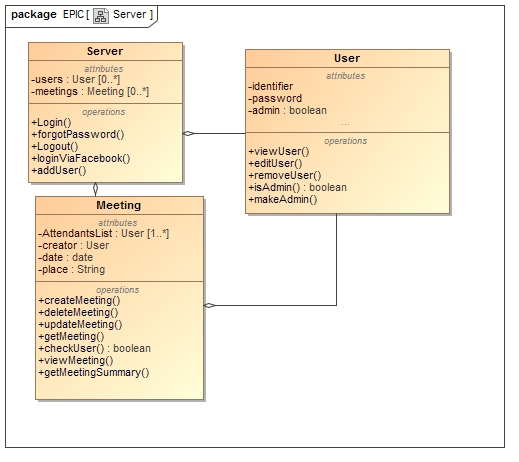
\includegraphics[width=0.8\textwidth]{ServerClass}
		 	 \caption{A Class Diagram of the Server}
		\end{figure}
		\subsubsection{Server}
			\begin{itemize}
			\item \textbf{Login}
				\newline\textbf{ Priority } - Critical
				\newline The user log into the system using a registered identifier and password, or the user may also log in via facebook.
	
		\begin{figure}[h!]	
 			 \centering
			  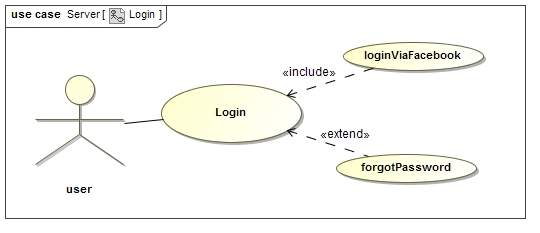
\includegraphics[width=0.8\textwidth]{LoginUseCase}
		 	 \caption{A Use Case Diagram of the Login services}
		\end{figure}
	
		\item \textbf{Logout}
				\newline\textbf{ Priority } - Critical
				\newline This service allows the user to log out if he is currently logged in.
			\item \textbf{addUser}
				\newline\textbf{ Priority } - Critical
				\newline The specified user is added to the system, but this service is only applicable to administrative users. 
			\end{itemize}
		\subsubsection{User}

		\begin{itemize}
			\item \textbf{isAdmin}
				\newline\textbf{ Priority } - Important
				\newline This service respond if the specified user is an administrative user.
			\item \textbf{makeAdmin}
				\newline\textbf{ Priority } - Important
				\newline Change the specified user to an administrative user. This service may only be done by another administrative user.

			\item \textbf{removeUser}
				\newline\textbf{ Priority } - Important
				\newline The specified user is removed from the system, but this service is only applicable to administrative users. 
			\item \textbf{viewUser}
				\newline\textbf{ Priority } - Important
				\newline View all the specified users data, but this service is only applicable to administrative users. 

		\end{itemize}

		\subsubsection{Meeting}
		\begin{itemize}
			\item \textbf{createMeeting}
				\newline\textbf{ Priority } - Critical
				\newline This service create a meeting. On creation the list of users attending the meeting must be added as well as the time and place of the meeting.
			\item \textbf{viewMeeting}
				\newline\textbf{ Priority } - Important
				\newline This service allows a user to view all the participants and the time and place of a meeting. An administrative user may view any meeting, but a common user may only view a meeting that they are attending.
			\item \textbf{updateMeeting}
				\newline\textbf{ Priority } - Important
				\newline This service allows the creator of the meeting or any administrative user to add or remove users to a meeting, as well as change the date, time or place.
			\item \textbf{deleteMeeting}
				\newline\textbf{ Priority } - Important
				\newline This service allows the creator of the meeting or any administrative user to delete a meeting.
			\item \textbf{getMeetingSummary}
				\newline\textbf{ Priority } - Important
				\newline This service give the user a list of all the users that attended the meeting as well as their entrance and exit times. This service is only active after the meeting has taken place.

		\end{itemize}

\newpage
		\subsection{Application}
			\textbf{Scope: }The Application is used when entering a meeting. The user will hold the android device over a gateway node. The application will send the identifier to the server via the Node and Gateway. The application will then, after confirmation from the Node, take a snapshot and enable the protection. After the meeting have occurred, the user will then hold the device over the Node again, the protection will be disabled and the phone will be stored to its previous state. 
		
		\begin{figure}[h!]
 			 \centering
			  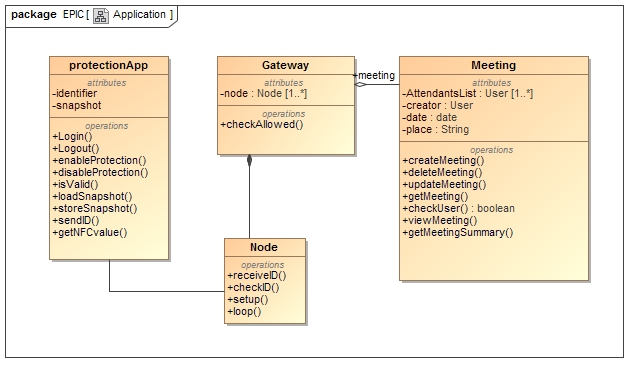
\includegraphics[width=0.8\textwidth]{ApplicationClass}
		 	 \caption{A Class Diagram of the protection Application, Meeting, Node and Gateway}
		\end{figure}

		\subsubsection{protectionApp}
		\begin{figure}[h!]
 			 \centering
			  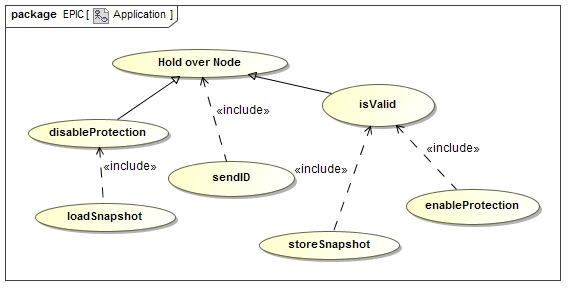
\includegraphics[width=0.8\textwidth]{ApplicationUseCase}
		 	 \caption{A Use Case Diagram protection Application}
		\end{figure}
		\begin{itemize}
			\item \textbf{login}
				\newline\textbf{ Priority } - Critical
				\newline The user login using his unique identifier and password. This service ensures that if the user use another device, his previous data is still intact.
			\item \textbf{logout}
				\newline\textbf{ Priority } - Critical
				\newline The user log out of the device.
			\item \textbf{SendID}
				\newline\textbf{ Priority } - Critical
				\newline Send identifier to the Node via NFC.
			\item \textbf{isValid}
				\newline\textbf{ Priority } - Critical
				\newline This service waits for respond from the Node for permission to  continue or halt. If the Node’s respond is to continue, storesnapshot is called and the protection is enabled.
			\item \textbf{enableProtection}
				\newline\textbf{ Priority } - Critical
				\newline The devices WiFi and GSM communication are turned off and the device go into silent mode.
			\item \textbf{storeSnapshot}
				\newline\textbf{ Priority } - Critical
				\newline A snapshot of the devices current networking state is stored.

			\item \textbf{loadSnapshot}
				\newline\textbf{ Priority } - Critical
				\newline The device is restored to the stored state.

			\item \textbf{getNFCvalue}
				\newline\textbf{ Priority } - Critical
				\newline When the NFC device is scanned it gets a value.


		\end{itemize}

\newpage		
		\subsection{Gateway and Node}
\textbf{Scope: }The Gateway consist of a Gateway and Nodes, connected in serial. The gateway node use NFC to communicate with the Android device. After the Android device is scanned the Node sends the identifier to the Gateway to see if the user may have access to the meeting and to update the meeting log. 

		\subsubsection{Node}

		\begin{itemize}
			\item \textbf{receiveID}
				\newline\textbf{ Priority } - Critical
				\newline Receive the identifier from the Android devices via NFC .
			\item \textbf{checkID}
				\newline\textbf{ Priority } - Critical
				\newline This service verify if the identifier may access the meeting on the Gateway. 
				\begin{figure}[h!]
 					 \centering
					  \includegraphics[width=0.8\textwidth]{CheckIDUseCase}
		 			 \caption{A Use Case Diagram of the CheckID service}
				\end{figure}
			\item \textbf{setup}
				\newline\textbf{ Priority } - Critical
				\newline Initialize everything
			\item \textbf{loop}
				\newline\textbf{ Priority } - Critical
				\newline run in a loop and call the receiveID service until an identifier is returned, it then call the checkID function.

		\end{itemize}

		\subsubsection{Gateway} The gateway receives the identifier from the node and verify the meeting access with the server. It also updates the meeting via the server.
		\begin{itemize}
			\item \textbf{getMeeting}
				\newline\textbf{ Priority } - Critical
				\newline Return the current meeting on loaded on the gateway device.
			\item \textbf{getAllowed}
				\newline\textbf{ Priority } - Critical
				\newline Return if the specified user is allowed in the meeting.
			

		\end{itemize}



\newpage
		
		\subsection{Malware}
		\textbf{Scope: } The malware consist of a webserver that connects with the mobile device via a web socket. A request is send from the server to the application on the mobile device to start recording. As the device records, the result is streamed directly to the server.
		\begin{figure}[h!]
 			 \centering
			  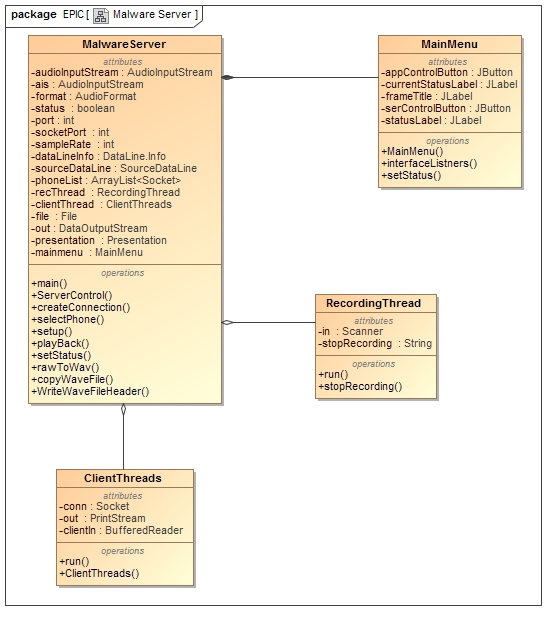
\includegraphics[width=0.8\textwidth]{MalwareClass}
		 	 \caption{A Class Diagram of the Malware}
		\end{figure}
	\subsubsection{Malware Server}
	With the server the user will be able to target a specific android device to start recording and streaming the data back to the server.
		\begin{figure}[h!]
 			 \centering
			  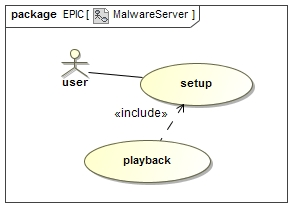
\includegraphics[width=0.6\textwidth]{MalwareServerUseCase}
		 	 \caption{A Use Case Diagram of the Malware Server}
		\end{figure}
		\begin{itemize}
			\item \textbf{sendStartRequest}
				\newline\textbf{ Priority } - Critical
				\newline This service send a request to start a recording to a specified device. If the device has the malware application installed and is reachable, the application will start streaming the recording to the server. If the device cannot be reached the service will send an error.
			\item \textbf{sendStopRequest}
				\newline\textbf{ Priority } - Critical
				\newline This service sends a request to the application on a specified device to stop the streaming and if it is currently storing the recording, stopStoreRecording is called.
			\item \textbf{playback}
				\newline\textbf{ Priority } - Critical
				\newline The recorded stream is played back to the user over the speakers.
			\item \textbf{setup}
				\newline\textbf{ Priority } - Critical
				\newline Initialize everything
		\end{itemize}	
		
\subsubsection{Malware Application}
	This application is hidden behind another application, but for the purpose of the project, the malware will be a visible application.
		\begin{figure}[h!]
 			 \centering
			  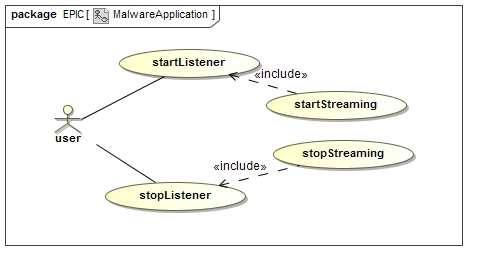
\includegraphics[width=0.8\textwidth]{MalwareApplicationUseCase}
		 	 \caption{A Use Case Diagram of the Malware Application}
		\end{figure}
		\begin{itemize}
			\item \textbf{startRecording}
				\newline\textbf{ Priority } - Critical
				\newline This service send a request to start a recording to a specified device. If the device has the malware application installed and is reachable, the application will start streaming the recording to the server. If the device cannot be reached the service will send an error.
			\item \textbf{stopRecording}
				\newline\textbf{ Priority } - Critical
				\newline This service stops the recording and stop streaming to the server.
			\item \textbf{startListener}
				\newline\textbf{ Priority } - Critical
				\newline The device listen for a request from the server to start the recording.
			\item \textbf{stopListener}
				\newline\textbf{ Priority } - Critical
				\newline The device listen for a request from the server to stop the recording.
			%\item \textbf{clientThread}
			%	\newline\textbf{ Priority } - Critical
			%	\newline 
		\end{itemize}

\end{document}